Early neuroanatomists had different ideas of how the brain was composed, some stated that it was a continuous organ, that is neurons were fused into a single mesh of cells with no separation. In the early 1900, Ramón y Cajal demonstrated that nervous system consisted of individual cells and that they communicated through different parts of their anatomy~\cite{Nemri:2010}. Figure~\ref{fig:neuro:ramon-y-cajal-neuro} shows one of his many drawings, it portraits neurons located near skin and muscular tissue.

\begin{figure}[hbt]
  \begin{center}
    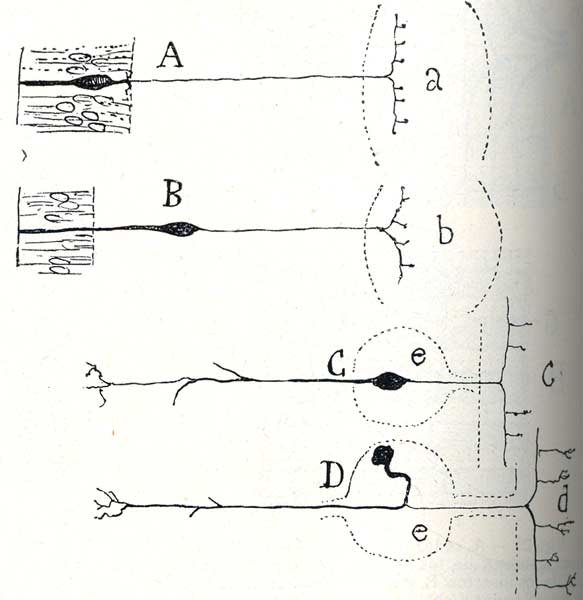
\includegraphics[width=0.45\textwidth]{ramon-y-cajal-fig_030}
    \caption{One of many Ramón y Cajal's drawings~\cite{cervantes-images}, it portraits neurons that are close to the skin and the muscles.}
    \label{fig:neuro:ramon-y-cajal-neuro}
  \end{center}
\end{figure}

These cells are called \emph{neurons} and they are particularly good at  long-range communication~\cite{thompson2000brain}. While most cells in the body can ``talk'' to their neighbours, neurons have structures that allow them to communicate for up to a meter~\cite{eye-brain-vision-hubel1995}. The flow of information through the billions of neurons in the brain is what originates behaviour, this is an amazing fact that has led many scientists to focus their minds into this phenomenon.

\subsection{Basic neural anatomy}

Neurons are composed of a \emph{soma} or body, this part has similar components to other cells in the body; and specialized communication structures called the \emph{axon} and \emph{dendrites}. The \textbf{neuron soma} has many similar elements to other cells in the human body (e.g. nucleus, mitochondria, Golgi apparatus). All the neuron is enclosed in the cell membrane, just like any other cell. The soma is the biggest shape at the left of Figure~\ref{fig:neuro:neuron-anatomy}. \textbf{Dendrites} are ramifications that come off the soma and, in most cases, are used as receivers of information from other neurons (red branch-like structures at the left of Figure~\ref{fig:neuro:neuron-anatomy}). The shape of dendrites allows the nerve cell to have a larger contact area for other cells to communicate with. For some neurons, dendritic branches have ``spines'', these are synapses formed with another neuron.

\begin{figure}
  \begin{center}
    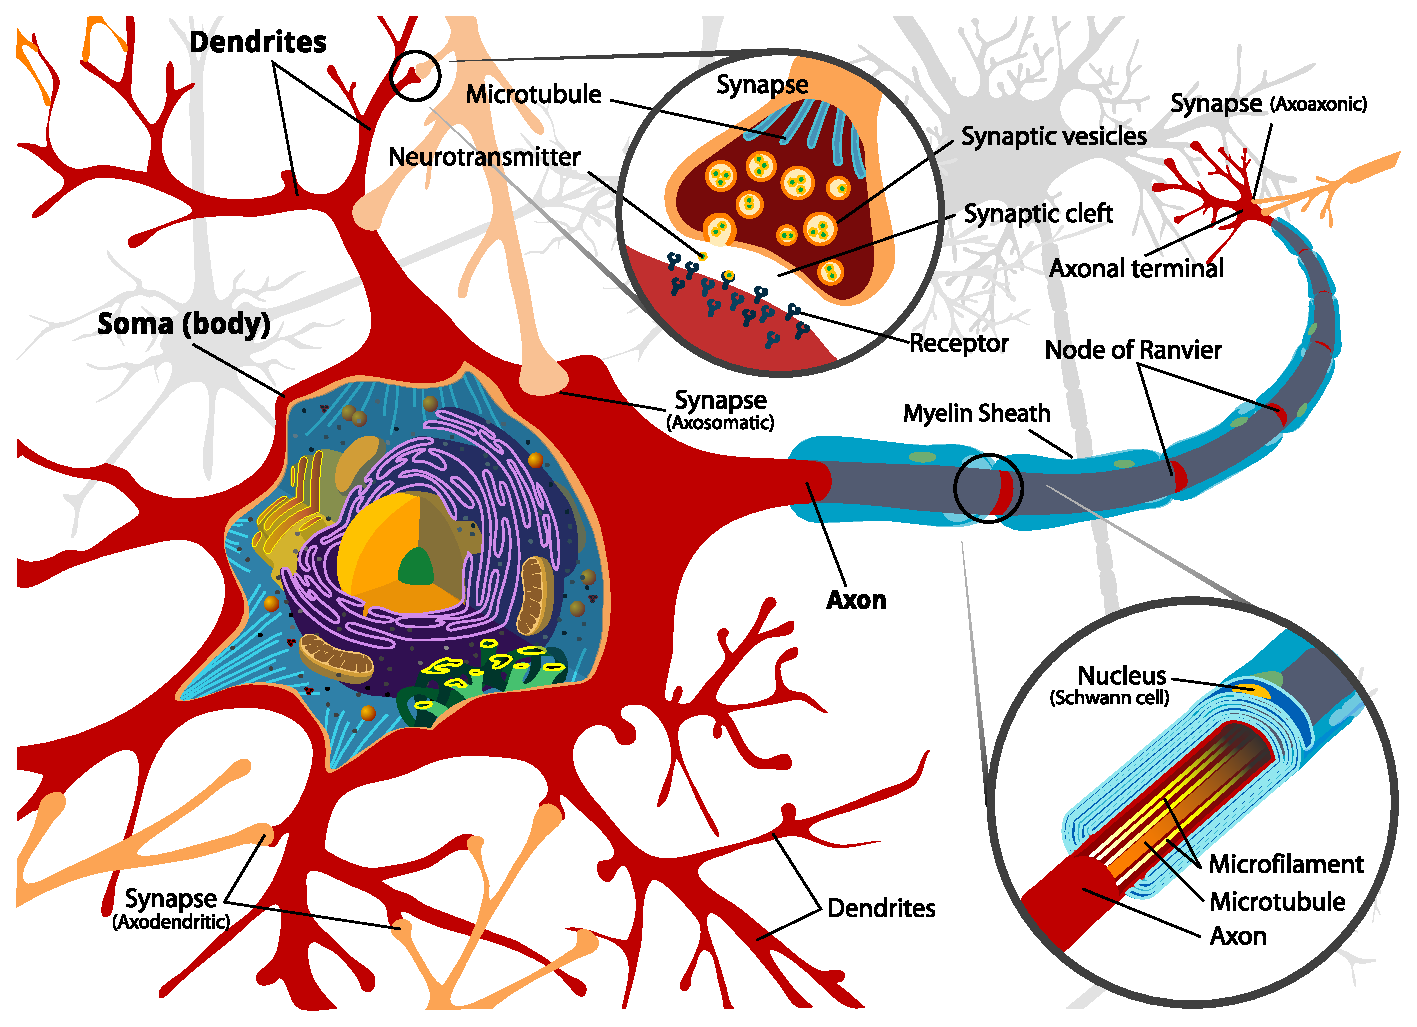
\includegraphics[width=\textwidth]{not-so-Complete_neuron_cell_diagram_en}
    \caption{Principal components of a neuron~\cite{wikipedia-images}.}
    \label{fig:neuro:neuron-anatomy}
  \end{center}
\end{figure}

The other specialized communication element of nerve cells is the \textbf{axon}, it's at the other end of the information exchange and can be seen as an output of the neuron. It usually has elongated tubular shape and ramifications at its end, shown at the right of Figure~\ref{fig:neuro:neuron-anatomy}. As with dendrites, the tree-like shape at the end of the axon permits larger contact area, thus, more neurons can interconnect. The middle portion of the axon may, sometimes, be covered by a thin layer \emph{myelin} (blue covering on the axon in Figure~\ref{fig:neuro:neuron-anatomy}); a substance that acts as an insulator and improves signal transmission~\cite{thompson2000brain}. Although this is the basic way nerve cells communicate, there are variations that have been recently discovered and are subject of new research efforts~\cite{Bullock04112005}.

The place where two cells are in proximity and information is exchanged is called the \textbf{synapse} (detail circle on top of Figure~\ref{fig:neuro:neuron-anatomy}). The cell sending information is labelled, \emph{pre-synaptic}; and the one receiving, \emph{post-synaptic}. The space between the pre- and post-synaptic cells is called the \emph{synaptic cleft} and it measures about $20 nm$. 

\subsection{Synapses}

Communication between neurons can be done through two types of processes, electrical and chemical, the latter being the most common in mammalian brains. In \textbf{chemical synapses}, the pre-synaptic neuron sends neurotransmitter molecules through pipes (\emph{microtubules}) that run inside its axon. At the end of the pre-synaptic axon, these transmitters are stored in vesicles. When a synapse is active, that is it's exchanging information, vesicles merge with the cell membrane and release the transmitters it stored.

When the pre-synaptic cell releases neurotransmitters, these will spread across the synaptic cleft. On the receiver end, the post-synaptic cell membrane is covered by chemical receptors of different types. After the release of transmitters from the pre-synaptic cell, chemical receptors in the post-synaptic neuron will receive them if they are of the right type. This exchange of chemicals will create a reaction on the receiving cell. One of the major differences between chemical and electrical synapses is that, the former ones are plastic, they can be changed throughout its formation to amplify or diminish its activity.

\textbf{Electrical synapses} are also known as \emph{gap junctions} and are thought to be rigid, it takes large changes in the cell to alter the synapse. This limits their information processing functionality because the way they are generated almost never changes. Gap junctions play an important role in most cells in the body, for example, they allow muscle cells to coordinate and create movement; researchers have found that they might also be critical for the development of the cortex~\cite{gap-junctions-pmid20066080,thompson2000brain}. 

%The receiving nerve cell might respond in two opposite manners, \emph{excitatory} and \emph{inhibitory}. 
The neuron membrane has an electrical potential with respect to the exterior fluid, it goes from -90 to +50~mV while resting. Chemical and electrical synapses alter this potential, pushing it towards a positive (excited, depolarized) or negative (inhibited, hyperpolarized) state. Figure~\ref{fig:neuro:exc_inh} shows the behaviour of the \emph{post-synaptic potential} (\textbf{PSP}) to the two types of inputs (excitatory first, then inhibitory). 

\begin{figure}[hbt]
  \begin{center}
    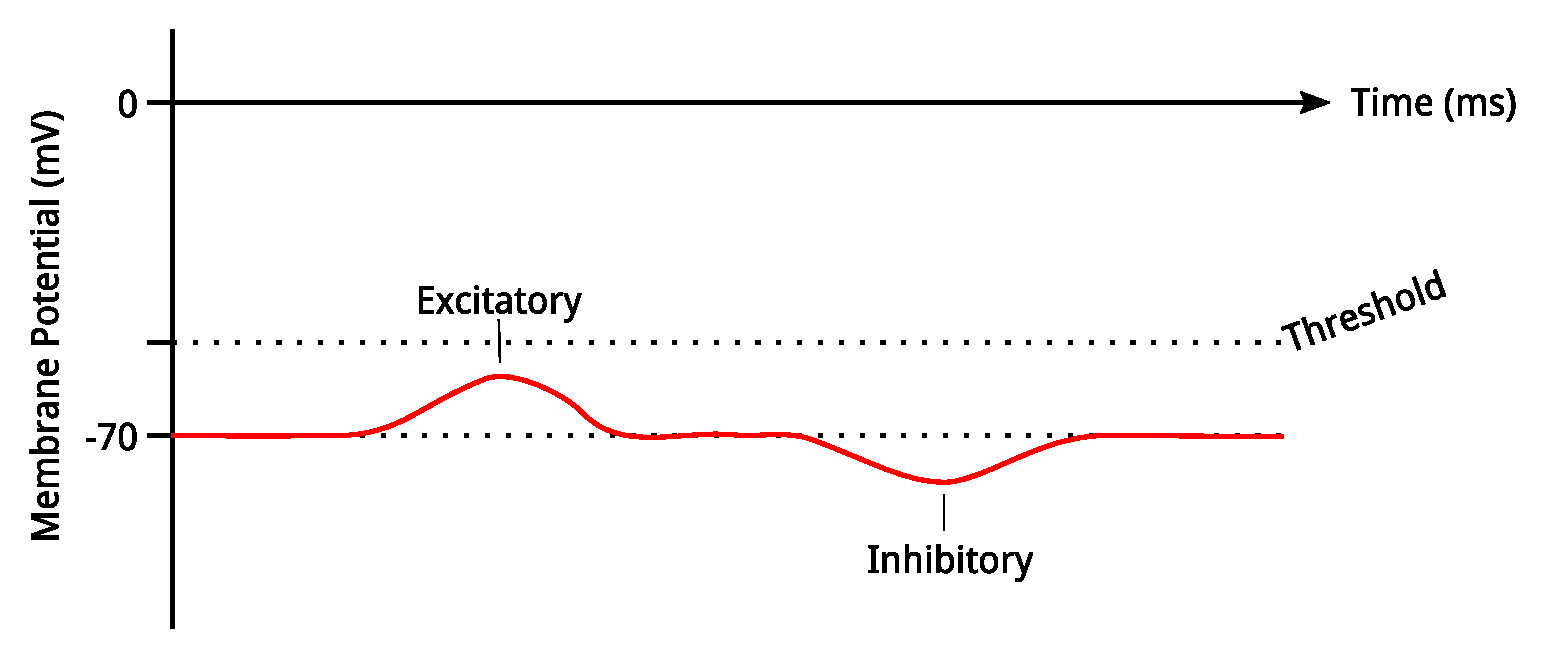
\includegraphics[width=0.8\textwidth]{excitation_inhibition}
    \caption{Post-synaptic membrane potential response to excitatory (left) and inhibitory (right) inputs.}
    \label{fig:neuro:exc_inh}
  \end{center}
\end{figure}

If the input is excitatory, the PSP will rise and have a better chance of generating an \emph{action potential} and its known as an \emph{excitatory post-synaptic potential} (\textbf{EPSP}). When the input is of the inhibitory kind, it will hyperpolarize the post-synaptic membrane potential; that is, it will diminish the probability of an action potential being generated. This type of response is known as \emph{inhibitory post-synaptic potential} (\textbf{IPSP}).

Whenever the membrane potential goes over a certain threshold (usually due to the accumulation of multiple EPSP), the neuron will generate an \textbf{action potential} also known as a \textbf{spike}. Figure \ref{fig:neuro:spike} shows an approximate graph of an action potential, each phase in the diagram is due to a change in ion concentration in the neuron (for a detailed explanation of this, see \cite{thompson2000brain}).

\begin{figure}[hbt]
  \begin{center}
    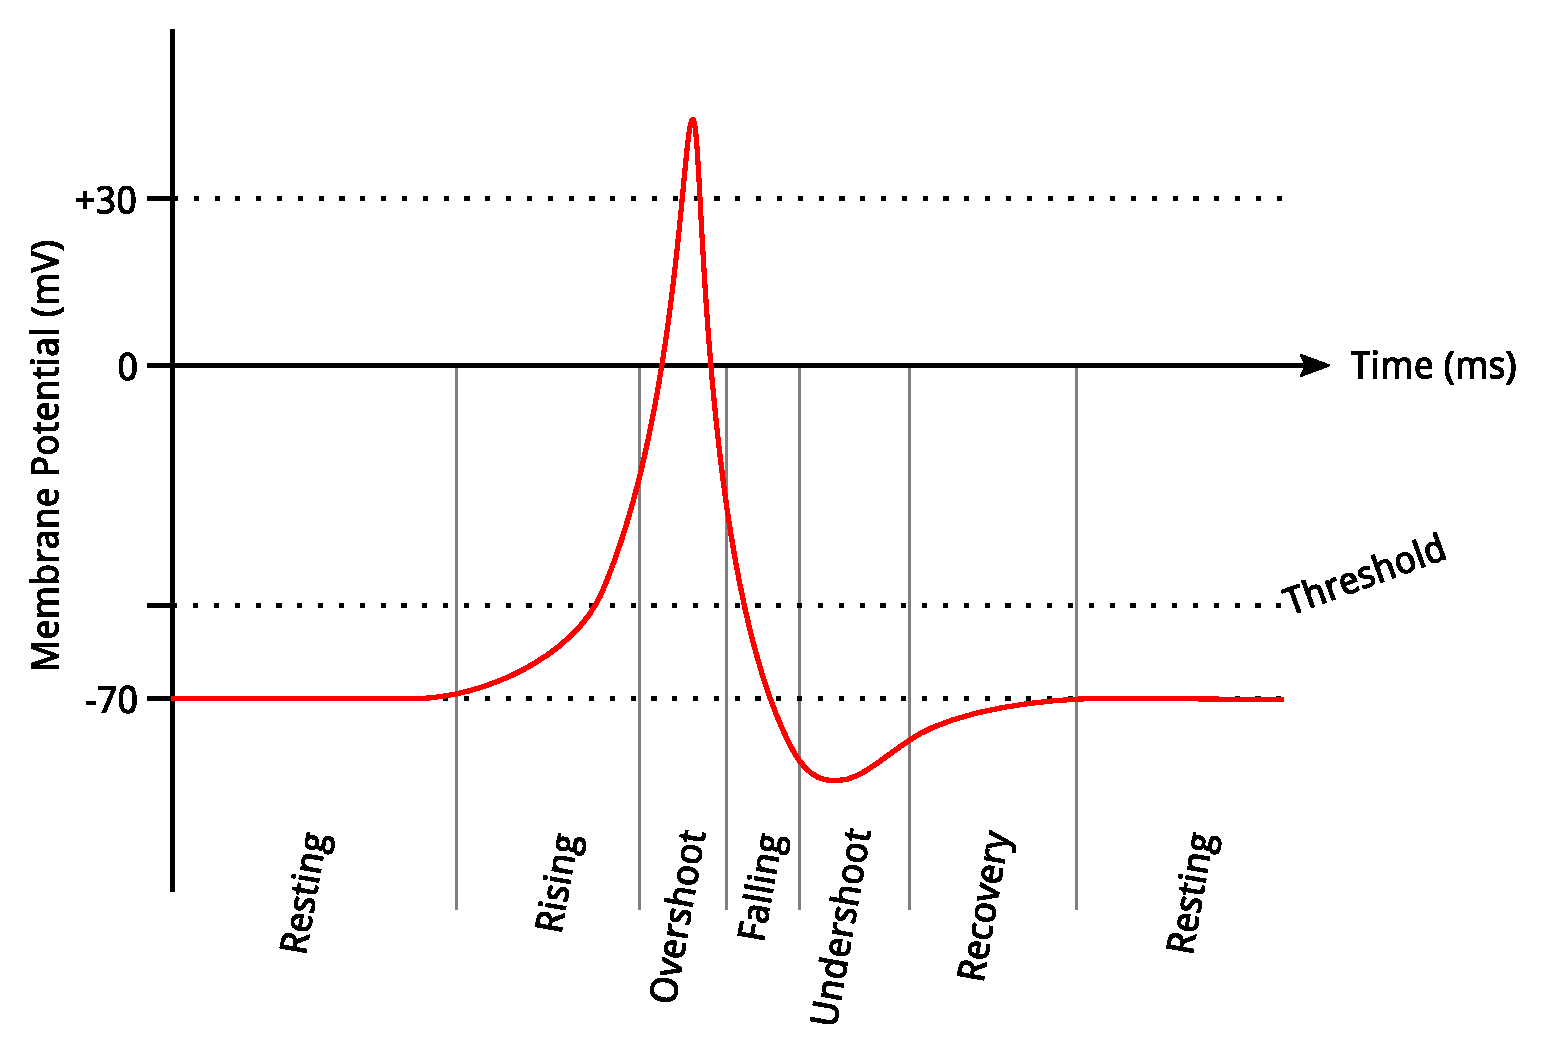
\includegraphics[width=0.8\textwidth]{action_potential}
    \caption{The action potential (spike) phases, each stage is associated with ion concentration changes in the neuron.}
    \label{fig:neuro:spike}
  \end{center}
\end{figure}

A spike is considered an \textsc{on}-or-\textsc{off} response from neurons and is thought to be the normal neural communication mechanism. Some neurons use analog/continuous signals to transmit information, though they are mostly found near sensory organs.

In summary, neurons receive information, in the form of action potentials, mostly through their dendrites. Nerve cells send information to other neurons through their axon; the space between axon and dendrite terminals is called the synapse. If action potentials increase the probability of the receiving neuron to generate a spike, then the potential came through an excitatory input. On the other hand, if it decreases the probability of spike generation, the potential came through an inhibitory synapse.

